\title{Answer Key for Calculus-Based Physics-1: Mechanics (PHYS150-01)}
\author{Dr. Jordan Hanson - Whittier College Dept. of Physics and Astronomy}
\date{December 13th, 2017}
\documentclass[10pt]{article}
\usepackage[a4paper, total={18cm, 27cm}]{geometry}
\usepackage{outlines}
\usepackage[sfdefault]{FiraSans}
\usepackage{graphicx}

\begin{document}
\maketitle

\section{Conceptual Questions}
\subsection{Kinematics and Angular Kinematics}
\begin{enumerate}
\item An object accelerates with constant acceleration.  The displacement versus time curve is quadratic.  The acceleration versus time plot should be $\rule{1cm}{0.15mm}$ and the velocity versus time plot should be $\rule{1cm}{0.15mm}$.
\begin{itemize}
\item quadratic, linear
\item linear, flat
\item \textbf{flat, linear}
\item linear, quadratic
\end{itemize}
\item An object experiences constant \textit{angular} acceleration.  The net external torque is $\rule{1cm}{0.15mm}$, and the angular velocity is a $\rule{1cm}{0.15mm}$ function of time.
\begin{itemize}
\item zero, linear
\item \textbf{constant, linear}
\item zero, constant
\item constant, constant
\end{itemize}
\item A battleship fires simultaneously two shells with the same speed at enemy ships (Fig. \ref{fig:battle}).  If the shells follow the parabolic trajectories shown, which ship gets hit first?
\begin{itemize}
\item A, because it has a smaller displacement from the cannon.
\item A, because the overall distance travelled is less.
\item Both at the same time, because the initial projectile velocity is the same.
\item \textbf{B, because the projectile does not have to travel as high in the air.}
\item B, because the initial velocity must be higher.
\end{itemize}
\begin{figure}[hb]
\centering
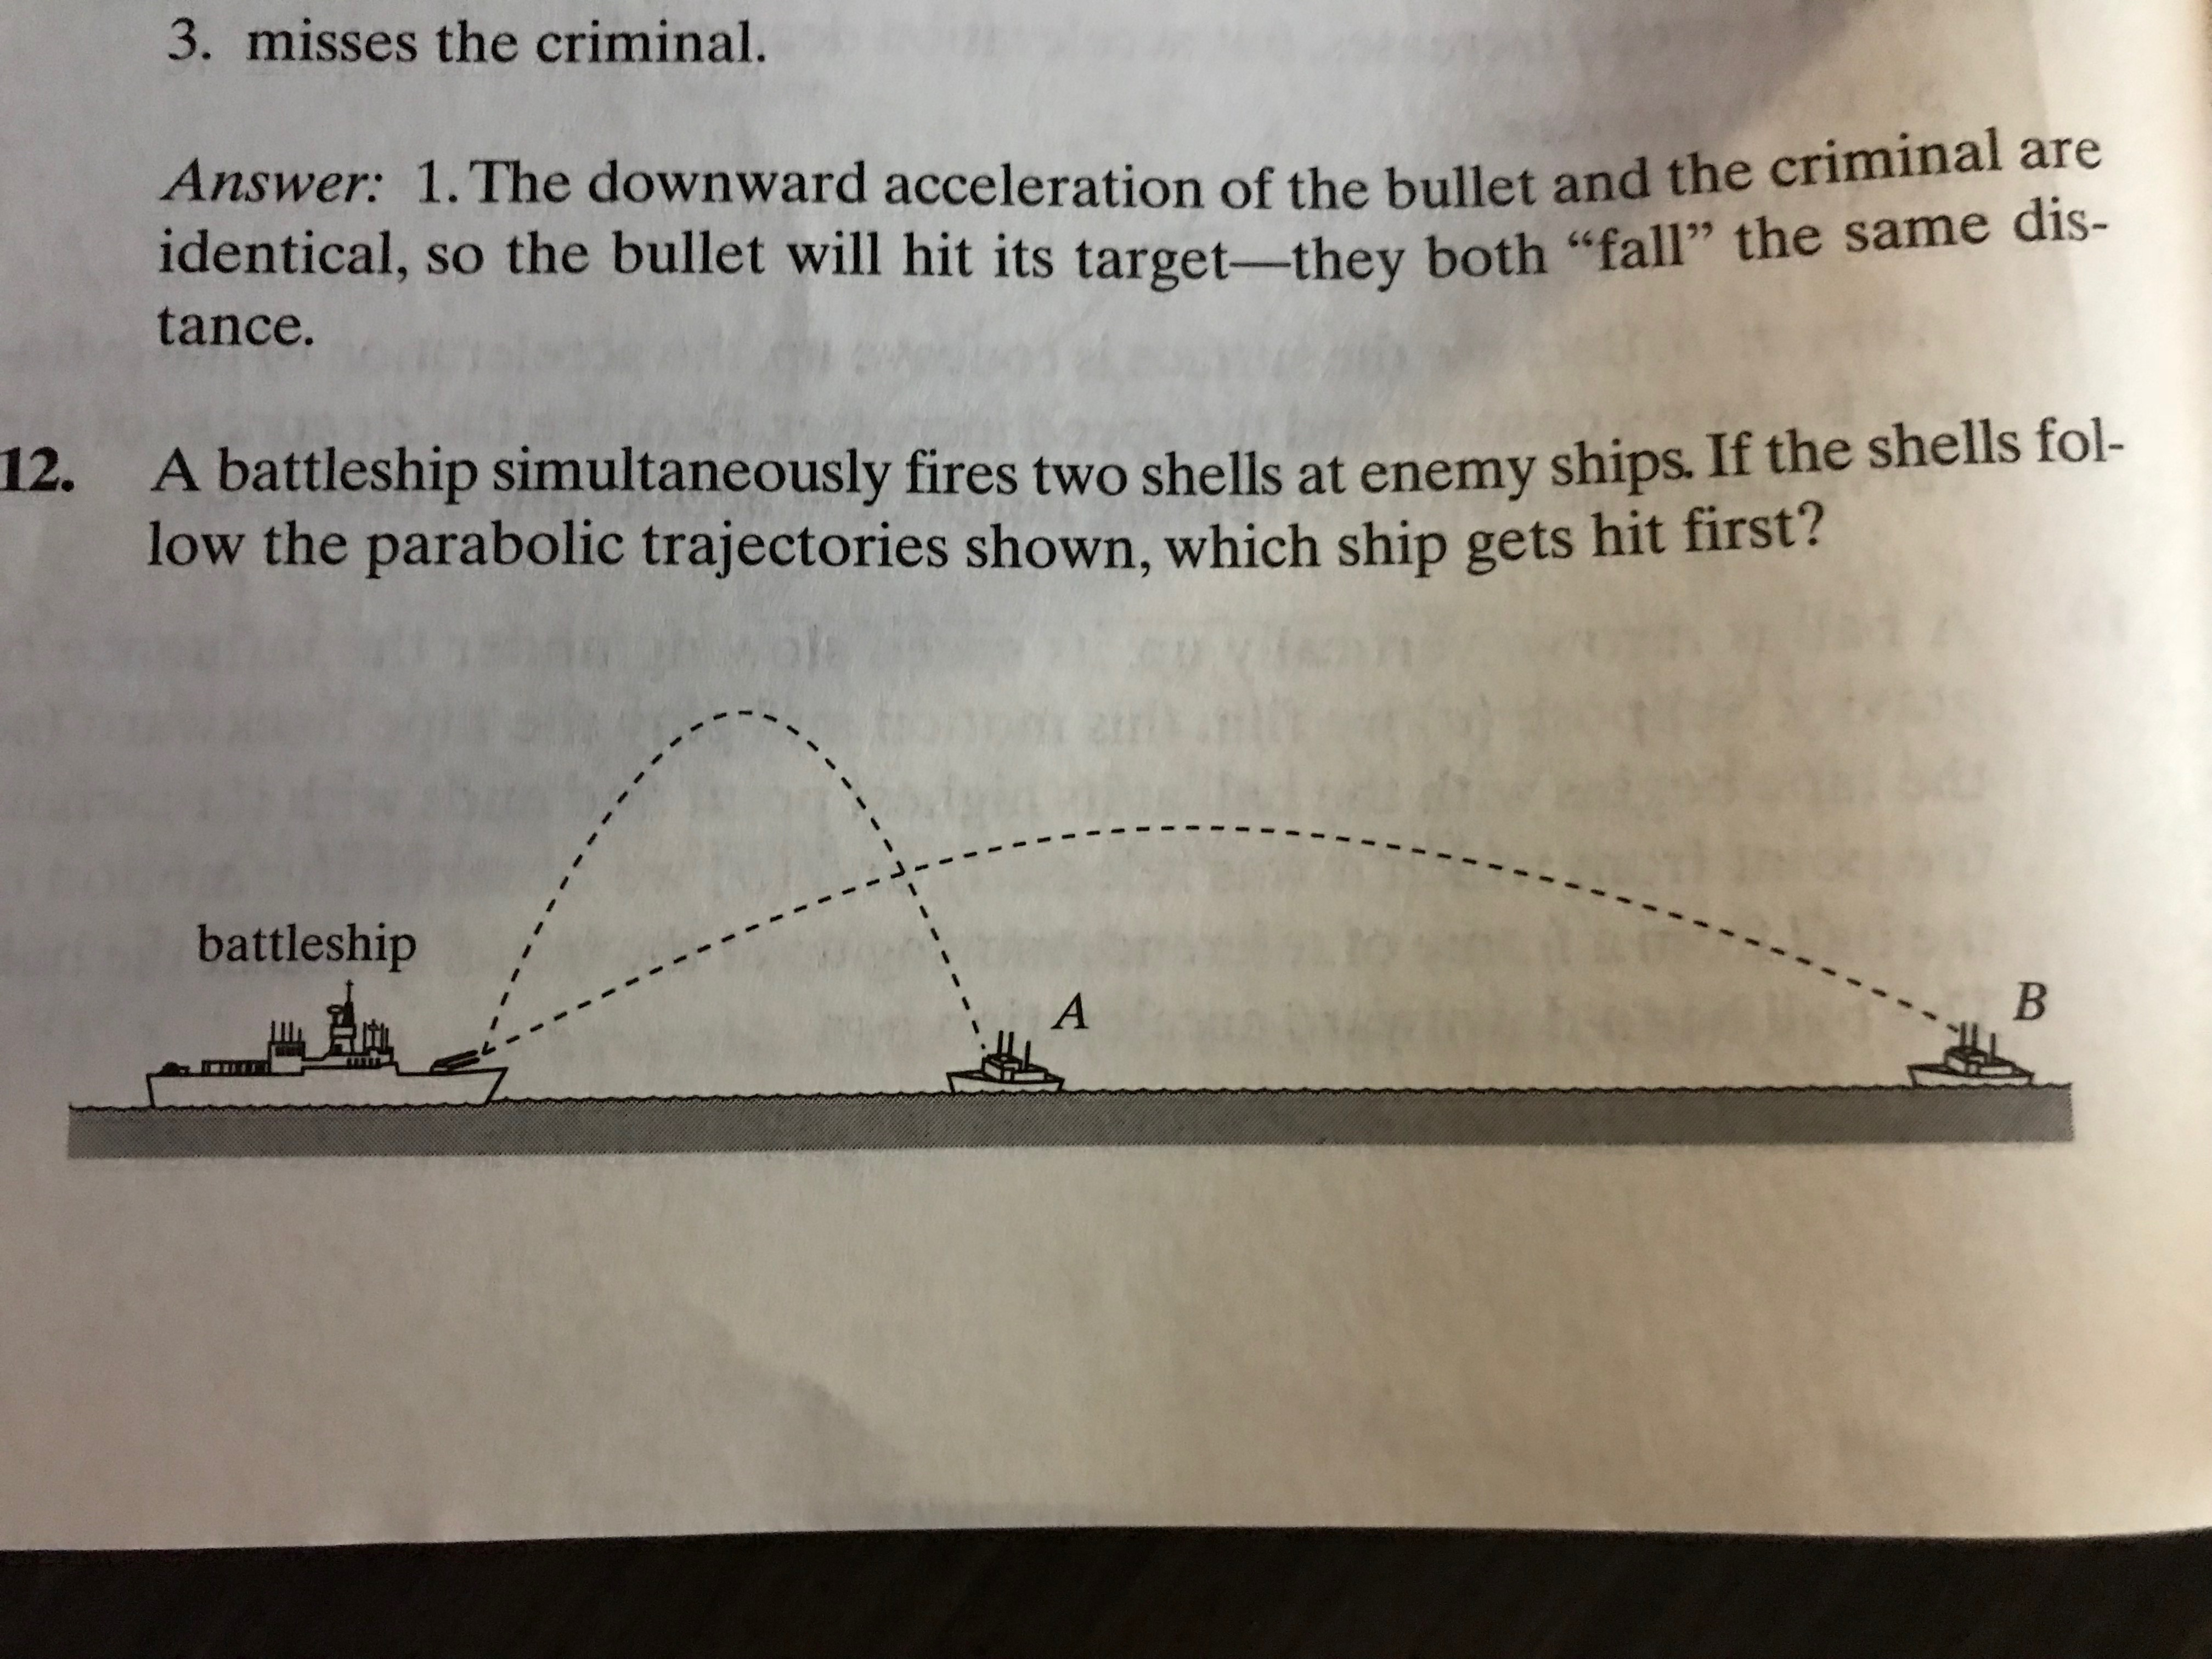
\includegraphics[width=0.6\textwidth,trim=0cm 30cm 0cm 45cm,clip=true]{battle.jpeg}
\caption{\label{fig:battle} Which ship is hit first?}
\end{figure}
\end{enumerate}
\subsection{Forces and Torque}
\begin{enumerate}
\item An elevator contains a person standing on a scale.  The elevator accelerates downward, then moves at constant velocity, then comes to a stop.  The scale reads a weight that is $\rule{1cm}{0.15mm}$, then $\rule{1cm}{0.15mm}$, and then $\rule{1cm}{0.15mm}$ the person's actual weight.
\begin{itemize}
\item More than, equal to, less than
\item \textbf{Less than, equal to, more than}
\item equal to, equal to, equal to
\item More than, equal to, equal to
\end{itemize}
\item A crate is pushed across a floor at constant velocity against friction.  The crate is flipped so that a side with less surface area is on the bottom.  If the required force to push it increases, which of the following is the proper conclusion?
\begin{itemize}
\item It's harder to push because there's more pressure now: pressure is force divided by area.
\item \textbf{It's harder to push because the new side must have a different coefficient of friction.}
\item It's harder to push because the normal force has increased.
\end{itemize}
\item A man needs to pull a rusty lever to release a mechanism, but he can't.  Which of the following will increase torque on the lever?
\begin{itemize}
\item Tying a rope to the end of the lever, and pulling on the rope perpendicular to the lever.
\item \textbf{Bolting a metal rod to the lever, and pulling the rod perpendicular to the lever.}
\item Tying a rope to the end of the lever, pulling the rope parallel to the lever.
\item Bolting a metal rod to the lever, and pulling the rod parallel to the lever.
\end{itemize}
\item An aircraft is in a banked turn, traveling in a circle.  Which of the following is most correct?
\begin{itemize}
\item \textbf{The craft experiences centripetal acceleration, provided by a component of the lift force.}
\item The craft experiences centripetal acceleration, provided by the thrust, which is tangent to the circle.
\item Moving at constant velocity, the craft experiences no acceleration.
\end{itemize}
\end{enumerate}
\subsection{Work and Energy}
\begin{enumerate}
\item In which of the follow situations would energy \textit{not} be conserved?
\begin{itemize}
\item An object is dropped from some height and experiences free-fall, neglecting air-resistance.
\item An external force compresses a mass against an oscillator for a given displacement and then the mass is released.
\item A pendelum is pulled away from equilibrium and then released.
\item \textbf{A train skids to a halt, with the wheels sliding on the tracks.}
\end{itemize}
\item A force does an amount of work $W$ on an object with initial velocity $v$ to stop it.  How much work would have to be done on the object if the initial velocity were $2v$?
\begin{itemize}
\item $2W$
\item $3W$
\item $4W$ \textbf{This one.}
\end{itemize}
\end{enumerate}
\subsection{Linear and Angular Momentum}
\begin{enumerate}
\item When a star undergoes a supernova, matter is blown away by a fusion reaction.  The more significant effect for angular momentum is that the star shrinks in size.  Suppose the radius decreases by a factor of $10^2$.  By what factor does the angular velocity increase, if angular momentum is conserved? (Assume the mass doesn't change significantly).
\begin{itemize}
\item 10$^3$
\item 10$^4$ \textbf{This one.}
\item 10$^5$
\end{itemize}
\item A mine cart holding two robbers is moving along a track at constant speed.  They're being chased, so one robber dives out the back.  The speed of the cart
\begin{itemize}
\item \textbf{increases, because momentum is conserved and the jumper has momentum in the opposite direction.}
\item decreases, because momentum is conserved and the mass of the cart has decreased.
\item remains constant, because there were only internal forces, not external forces.
\end{itemize}
\item If ball 1 in the arrangement shown in Fig. \ref{fig:newton} is pulled back and then let go, ball 5 bounces forward.  If balls 1 and 2 are pulled back and released, balls 4 and 5 bounce forward, and so on.  The number of balls bouncing on each side is equal because
\begin{itemize}
\item of conservation of momentum.
\item \textbf{the collisions are elastic.}
\item the collisions are inelastic.
\item neither of the above.
\end{itemize}
\begin{figure}
\centering
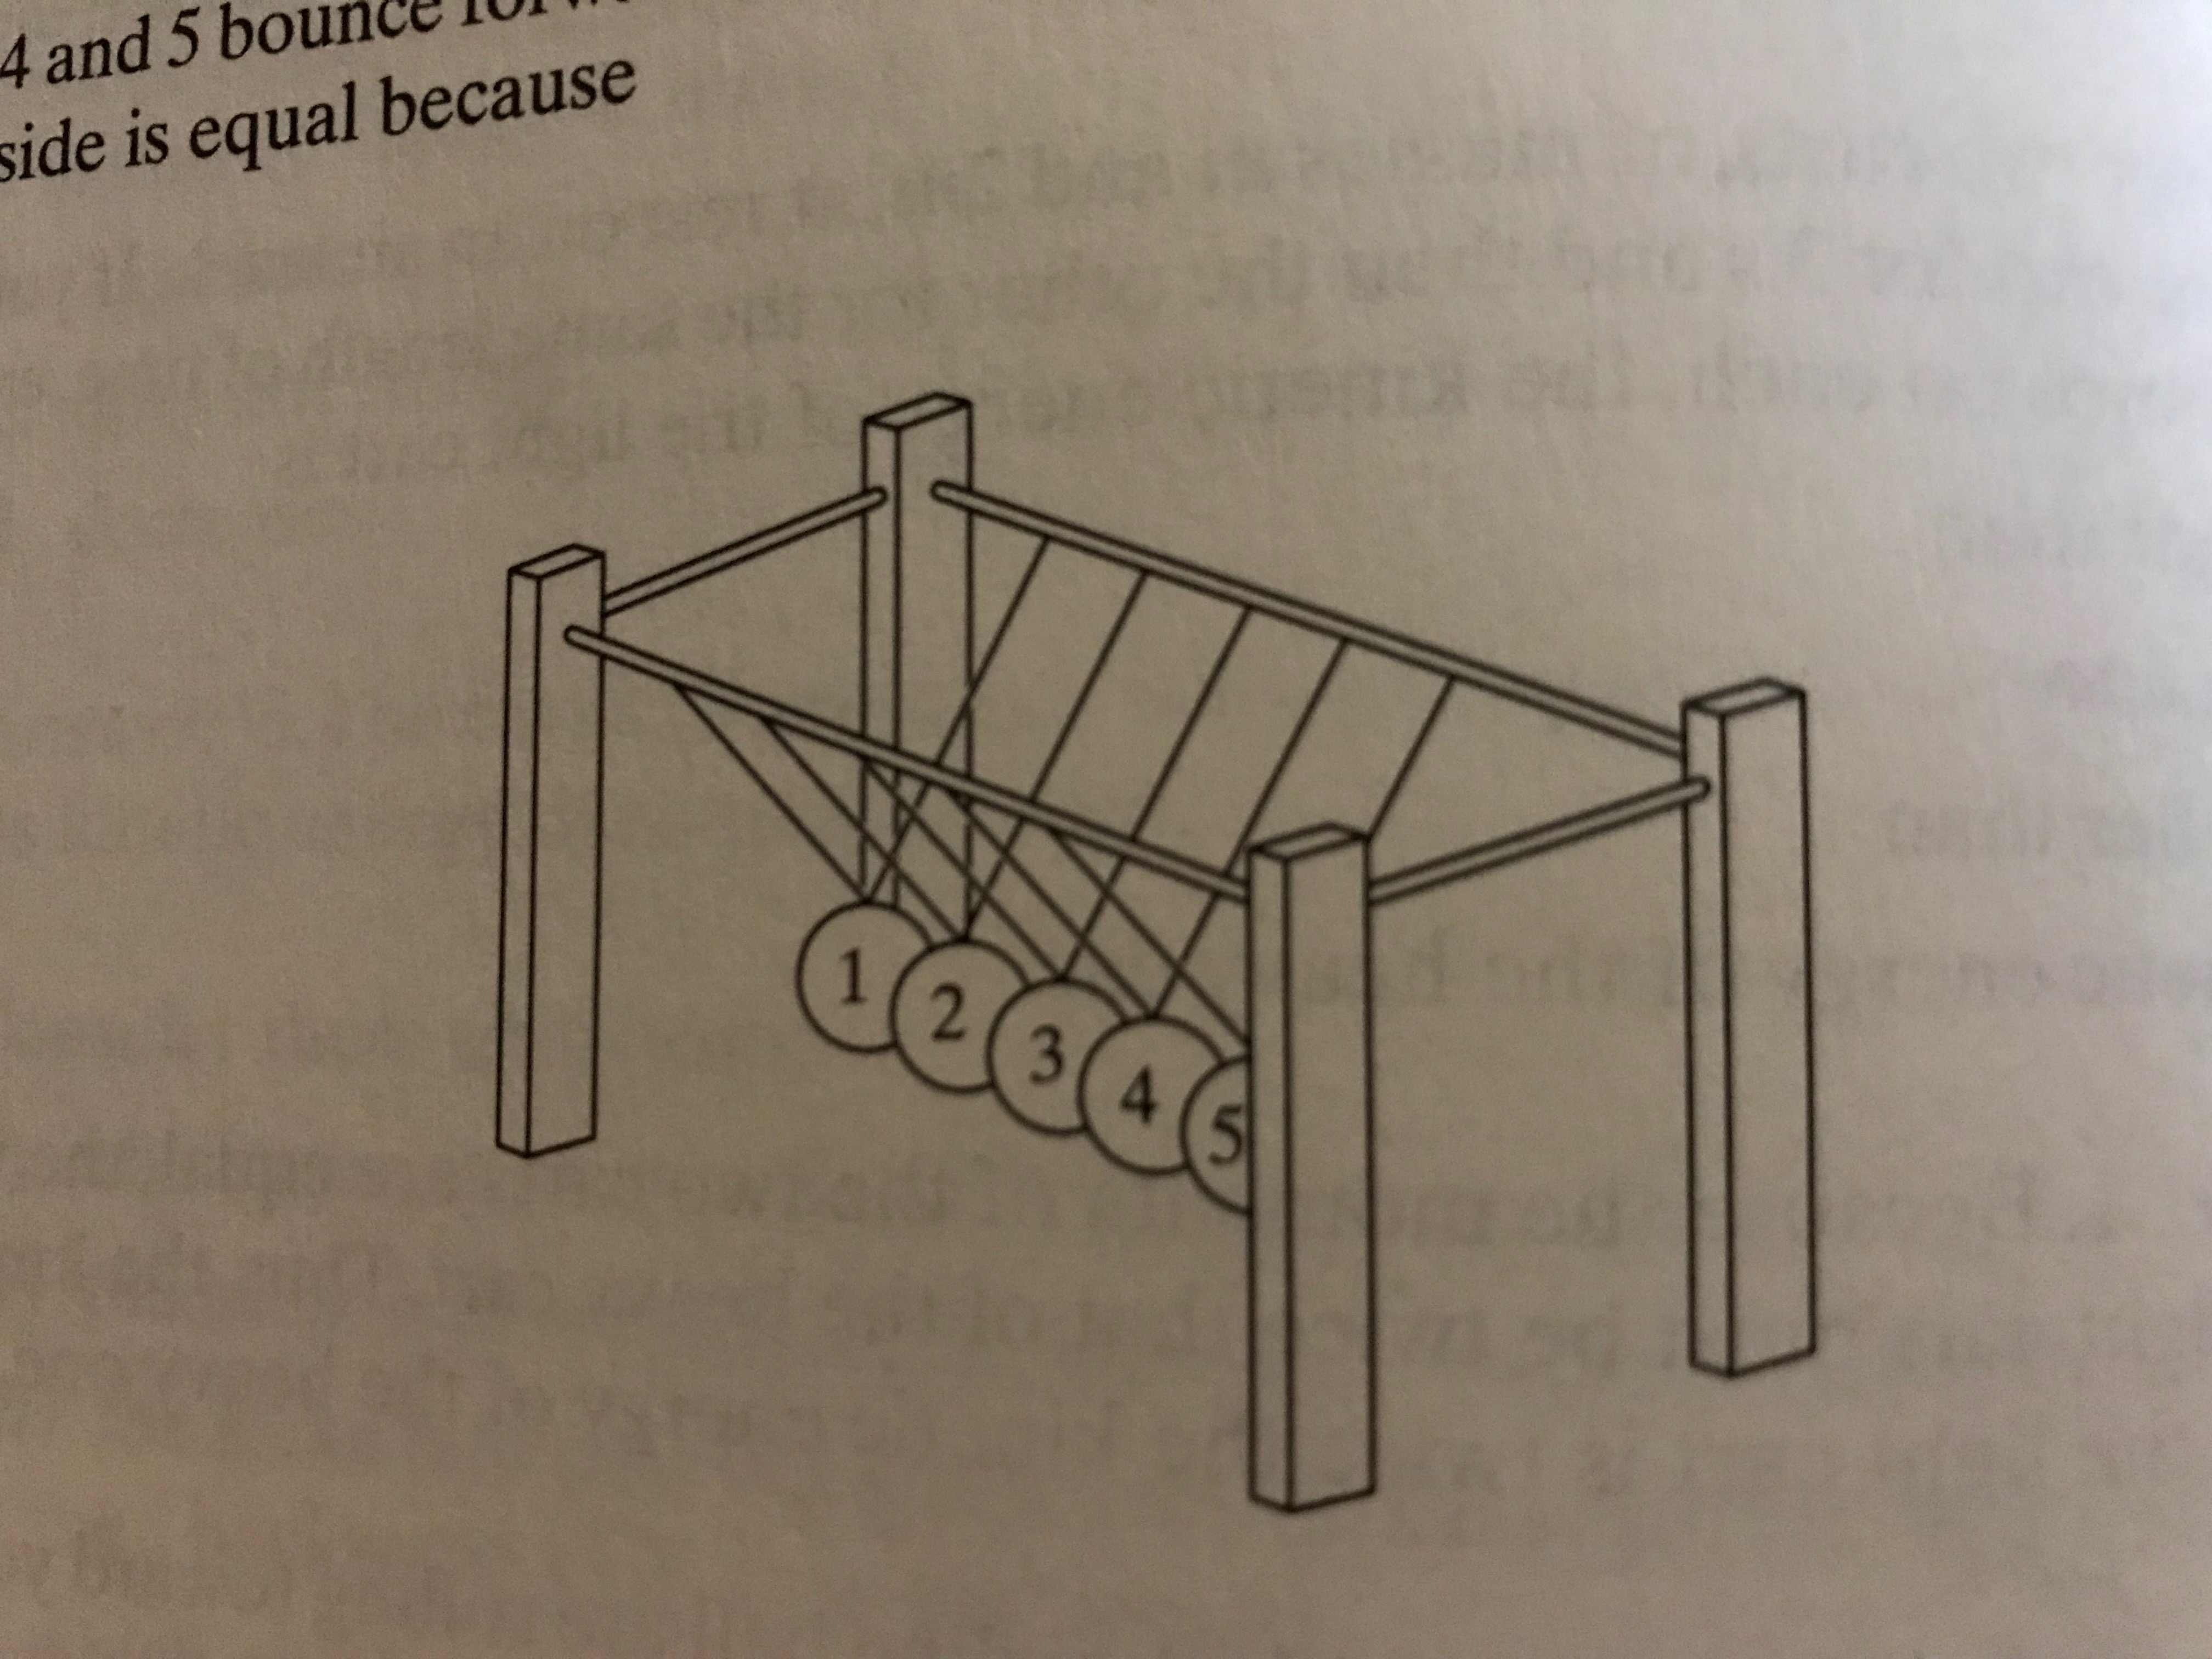
\includegraphics[width=0.2\textwidth,trim=20cm 5cm 15cm 20cm,clip=true]{newton.jpeg}
\caption{\label{fig:newton} This object is known as a Newton's cradle.}
\end{figure}
\end{enumerate}
\section{Technical Questions}
\subsection{Kinematics and Angular Kinematics}
\begin{enumerate}
\item A ball is kicked with an initial velocity of $\vec{v} = 3\hat{i}+4\hat{j}$ m/s. (a) For how long does the ball remain in the air?  (b) Where does the ball land? ($g=10$ m/s$^2$). ($\frac{1}{3}$ point for correct diagram, $\frac{2}{3}$ point for numerical answers). \\ \\
The diagram is a concave-down parabola.  (a) $v_{\rm y}(t) = v_{\rm y,i} - gt$.  The total time is therefore $t = 2v_{\rm y,i}/g = 4/5$ seconds.  (b) $\Delta x = v_{\rm x,i}t = 3(4)/5 = 12/5$ meters.
\end{enumerate}
\subsection{Forces and Torque}
\begin{enumerate}
\item A 900 kg lunar probe hovers above the surface of the Moon.  On the Moon, $g \approx 5/3$ m/s$^2$.  An engine is pointed at a 30 degree angle from straight down, spraying propellant.  What force does the engine produce to keep the probe from decreasing in height?  ($\frac{1}{3}$ point for correct free-body diagram, $\frac{2}{3}$ point for answer).  \\ \\
The free body diagram contains two forces, the weight downward and the thrust upwards, 30 degrees from vertical.  From the free-body diagram, we find to balance the forces, we need $T = w/\cos\theta = mg/\cos\theta = 3000/\sqrt{3}$ N.
\end{enumerate}
\subsection{Work and Energy}
\begin{enumerate}
\item A snowboarder descends a hill with a height of 25 meters (neglect friction).  (a) What is her final speed?  (b) After descending, she travels along a flat stretch of snow.  She turns the board sideways, the coefficient of friction becomes relevant: $\mu = 0.5$.  How far does she travel before stopping? \\ \\
From energy conservation, we find $v = \sqrt{2gh} = \sqrt{500} = 10\sqrt{5}$ m/s.  (b) The acceleration is $a = \mu g$, so kinematically, $\Delta x = v^2/(2\mu g) = 50$ meters.
\end{enumerate}
\subsection{Linear and Angular Momentum}
\begin{enumerate}
\item Two objects each of mass $m = 0.2$ kg rotate around the origin of a coordinate system, both at radius $r = 0.2$ m.  If the tangential velocity of each is $v = 2$ m/s ($p = mv$), (a) what is $L = L_1 + L_2 = r_1 p_1\sin\theta_1+r_2 p_2\sin\theta_2$, the total angular momentum?  (b) What is the value of the total \textit{moment of inertia}, $I = 2mr^2$, and the \textit{angular speed} $\omega = v/r$ of the particles?  (c) Show numerically that $I\omega = L$ from part (a). \\ \\
(a) $L = (2)2\frac{2}{10}\frac{2}{10}(1) = \frac{4}{25}$ J s (the two objects have the same angular momentum).  (b) $I = 2mr^2 = 2\frac{2}{10}\frac{4}{100} = \frac{16}{1000}$ kg m$^2$. $\omega = v/r = 2/\frac{2}{10} = 10$ rad/second.  (c) Thus, $I\omega = \frac{16}{1000}10 = \frac{4}{25}$ J s.
\begin{figure}[hb]
\centering
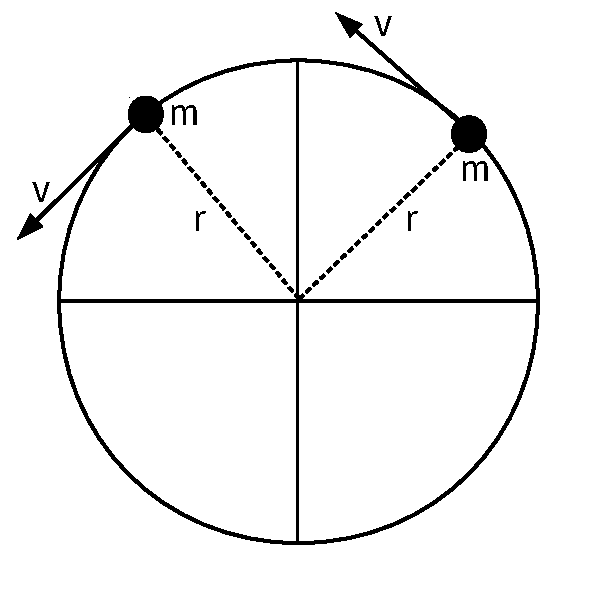
\includegraphics[width=0.2\textwidth]{rotate.pdf}
\end{figure}
\end{enumerate}
\end{document}